\section{A Baseline} \label{sec:baseline}

To get a feeling for how good or bad the results for minimizing wirelength based on NLSE or NWA are,
we will start by evaluating them with the following parameters:
\begin{itemize}
 \item Start vector: RANDOM
 \item Optimization method: Nesterov's accelerated gradient method
 \item The step size strategy: \texttt{backtracking-line-search}
 \item The stopping criterion: After exactly 1000 iterations
\end{itemize}
While the random start vector is presumably not very close to the optimum,
it also has no inherent structure that could accelerate or decelerate the convergence of the optimization methods.
The optimization method was chosen to be NAG with \texttt{backtracking-line-search} because it is reliable and fast.
It was shown by Nesterov in \cite{Nesterov-NesterovAcceleratedGradient} that this method has a similar convergence guarantee
as using a constant step size of \(1/L\) (see \cref{thm:nesterovs_accelerated_gradient_converges}).
Lastly, we chose to run for 1000 iterations, a very high number, to test what this method is capable of.

All of the following graphs and plots were produced by runs on a rather large chip which we will call \texttt{Chip1}.
It has roughly 2,000,000 movable cells, 5,600,000 pins and 2,000,000 nets.
The placement area of this chip is about 1.3 millimeter wide and 0.9 millimeter high.

\begin{figure}[t]
 \centering
 \begin{tikzpicture}
  \begin{groupplot} [
      width=(\textwidth-1cm),
      height=(\textwidth-1cm)/2,
      group style={group size=1 by 2},
      group/xlabels at=edge bottom,
      xlabel=Iteration,
      ylabel=Objective function,
      y unit=\si{\meter},
      enlarge x limits={value=0.05, upper},
      xmin=0,
%       xmax=1000,
      restrict y to domain=0:500,
      ymax=400,
  ]
   \nextgroupplot
   \addlegendentry{\(T_{\NLSE_\gamma}\) with \(\gamma = 10^1\)}
   \addplot [blue, thick] table [
     x=iteration,
     y=LSE_10_gamma_objective,
   ] {chapters/results/baseline/convergence_Chip1_by_gamma.data};
  
   \addlegendentry{\(T_{\NLSE_\gamma}\) with \(\gamma = 10^3\)}
   \addplot [dark_green, thick] table [
     x=iteration,
     y=LSE_1000_gamma_objective,
   ] {chapters/results/baseline/convergence_Chip1_by_gamma.data};

   \addlegendentry{\(T_{\NLSE_\gamma}\) with \(\gamma = 10^5\)}
   \addplot [red, thick] table [
     x=iteration,
     y=LSE_100000_gamma_objective,
   ] {chapters/results/baseline/convergence_Chip1_by_gamma.data};

   \addlegendentry{HPWL of \(T_{\NLSE_\gamma}\) with \(\gamma = 10^5\)}
   \addplot [red, dashed, thick] table [
     x=iteration,
     y=LSE_100000_gamma_hpwl,
   ] {chapters/results/baseline/convergence_Chip1_by_gamma.data};

   \nextgroupplot
   \addlegendentry{\(T_{\NWA_\gamma}\) with \(\gamma = 10^1\)}
   \addplot [blue, thick] table [
     x=iteration,
     y=WA_10_gamma_objective,
   ] {chapters/results/baseline/convergence_Chip1_by_gamma.data};

   \addlegendentry{\(T_{\NWA_\gamma}\) with \(\gamma = 10^3\)}
   \addplot [dark_green, thick] table [
     x=iteration,
     y=WA_1000_gamma_objective,
   ] {chapters/results/baseline/convergence_Chip1_by_gamma.data};

   \addlegendentry{\(T_{\NWA_\gamma}\) with \(\gamma = 10^5\)}
   \addplot [red, thick] table [
     x=iteration,
     y=WA_100000_gamma_objective,
   ] {chapters/results/baseline/convergence_Chip1_by_gamma.data};

   \addlegendentry{HPWL of \(T_{\NWA_\gamma}\) with \(\gamma = 10^5\)}
   \addplot [red, dashed, thick] table [
     x=iteration,
     y=WA_100000_gamma_hpwl,
   ] {chapters/results/baseline/convergence_Chip1_by_gamma.data};

  \end{groupplot}
 \end{tikzpicture}
 \caption{Objective function by iteration of NAG depending on \(\gamma\)} 
 \label{fig:baseline_objective_function_convergence_by_gamma}
\end{figure}

For the graphs in \cref{fig:baseline_objective_function_convergence_by_gamma}
we optimized \(T_{\NLSE_\gamma}\) and \(T_{\NWA_\gamma}\) for different values of \(\gamma\)
and graphed the value of the objective function that was used by iteration.
Note that even though x- and y-direction were optimized independently, we added up the values of the objective functions
for both directions to get an overall picture of the progress.
Because it is also interesting to see how \(T_{\HPWL}\) develops for each of these
runs, the dashed red line was added for \(\gamma = 10^5\).
For the other two \(\gamma\)-values, \(T_{\HPWL}\) is so close to the objective function 
that the differences are not visible in the plots so these lines were omitted.

What conclusions can be drawn from these pictures?
Nesterov's accelerated gradient method is able to optimize \(T_{\NLSE_\gamma}\) and \(T_{\NWA_\gamma}\) successfully.
All six objective functions where minimized such that \(T_{\HPWL}\) decreased to similar values.
This is also true for \(\gamma = 10^5\) where a significant difference between the objective functions
and \(T_{\HPWL}\) can be seen.
How the different final placements compare when evaluated by different objective functions will be investigated later.
When comparing the pictures for \(\NLSE\) and \(\NWA\) the similarity is striking.
For \(\gamma \leq 10^3\) this is explained by the fact that all of the objective functions
are already very close to \(T_{\HPWL}\) and therefore close to each other.
Regarding \(T_{\NLSE_\gamma}\) and \(T_{\NWA_\gamma}\) with \(\gamma = 10^5\),
the latter is indeed closer the HPWL objective function as predicted by \cref{thm:NWA_approximates_HPWL_better_than_NLSE}
but the dashed red lines are very similar,
so their success at minimizing linear netlength is comparable.

\begin{figure}[t]
 \centering
 \begin{tikzpicture}
  \begin{groupplot} [
      width=(\textwidth-1cm),
      height=(\textwidth-1cm)/2,
      group style={group size=1 by 2},
      group/xlabels at=edge bottom,
      xlabel=Iteration,
      ylabel=Gradient norm,
      y unit=\si{\micro\meter},
      enlarge x limits={value=0.05, upper},
      xmin=0,
  ]
   \nextgroupplot
   \addlegendentry{\(\norm{\nabla T_{\NLSE_\gamma}}_2\) with \(\gamma = 10^1\)}
   \addplot [blue, thick] table [
    x=iteration,
    y=LSE_10_gamma_euclidean_norm,
   ] {chapters/results/baseline/convergence_Chip1_by_gamma.data};

   \addlegendentry{\(\norm{\nabla T_{\NLSE_\gamma}}_2\) with \(\gamma = 10^3\)}
   \addplot [dark_green, thick] table [
    x=iteration,
    y=LSE_1000_gamma_euclidean_norm,
   ] {chapters/results/baseline/convergence_Chip1_by_gamma.data};

   \addlegendentry{\(\norm{\nabla T_{\NLSE_\gamma}}_2\) with \(\gamma = 10^5\)}
   \addplot [red, thick] table [
    x=iteration,
    y=LSE_100000_gamma_euclidean_norm,
   ] {chapters/results/baseline/convergence_Chip1_by_gamma.data};

   \nextgroupplot
   \addlegendentry{\(\norm{\nabla T_{\NWA_\gamma}}_2\) with \(\gamma = 10^1\)}
   \addplot [blue, thick] table [
    x=iteration,
    y=WA_10_gamma_euclidean_norm,
   ] {chapters/results/baseline/convergence_Chip1_by_gamma.data};

   \addlegendentry{\(\norm{\nabla T_{\NWA_\gamma}}_2\) with \(\gamma = 10^3\)}
   \addplot [dark_green, thick] table [
    x=iteration,
    y=WA_1000_gamma_euclidean_norm,
   ] {chapters/results/baseline/convergence_Chip1_by_gamma.data};

   \addlegendentry{\(\norm{\nabla T_{\NWA_\gamma}}_2\) with \(\gamma = 10^5\)}
   \addplot [red, thick] table [
    x=iteration,
    y=WA_100000_gamma_euclidean_norm,
   ] {chapters/results/baseline/convergence_Chip1_by_gamma.data};

  \end{groupplot}
 \end{tikzpicture}
 \caption{Gradient norm by iteration of NAG depending on \(\gamma\)} 
 \label{fig:baseline_gradient_convergence_by_gamma}
\end{figure}

To investigate the convergence properties of these objective functions,
we can take a look at the Euclidean norm 
of the gradients for each NAG iteration of each of these different optimization processes
in \cref{fig:baseline_gradient_convergence_by_gamma}.
Even though x- and y-direction were optimized independently, the Euclidean norms
were added up for both directions to get an overall picture of the progress.
Looking at the graphs for each direction individually shows very similar lines.
As discussed in \cref{subsec:stopping_criterion}, the norm of the gradient serves as an indication
of how close the optimization process is to reaching the optimum.
Only for the highest \(\gamma\)-value of \(10^5\) a clear decrease down to zero can be seen.
This is an important property because if the gradient norm does not converge to zero,
the stopping criterion will not work correctly.
It was expected that lower \(\gamma\)-values would lead to worse convergence properties
because the Lipschitz constant of the objective functions are higher
but it was not clear how big this impact would be.
The given graph indicates that they are so bad that \(\gamma\)-values lower than \(10^5\)
cannot be handled by the chosen convex optimization techniques very well.
When comparing \(\NLSE_\gamma\) and \(\NWA_\gamma\) using \(\gamma = 10^5\),
the gradient of the latter does converge slower to zero than the gradient of the former:
Using the same \(\gamma\)-value \(\NLSE_\gamma\) converges faster than \(\NWA_\gamma\).

\begin{figure}[p]
 \centering
 \begin{subfigure}{.48\textwidth}
  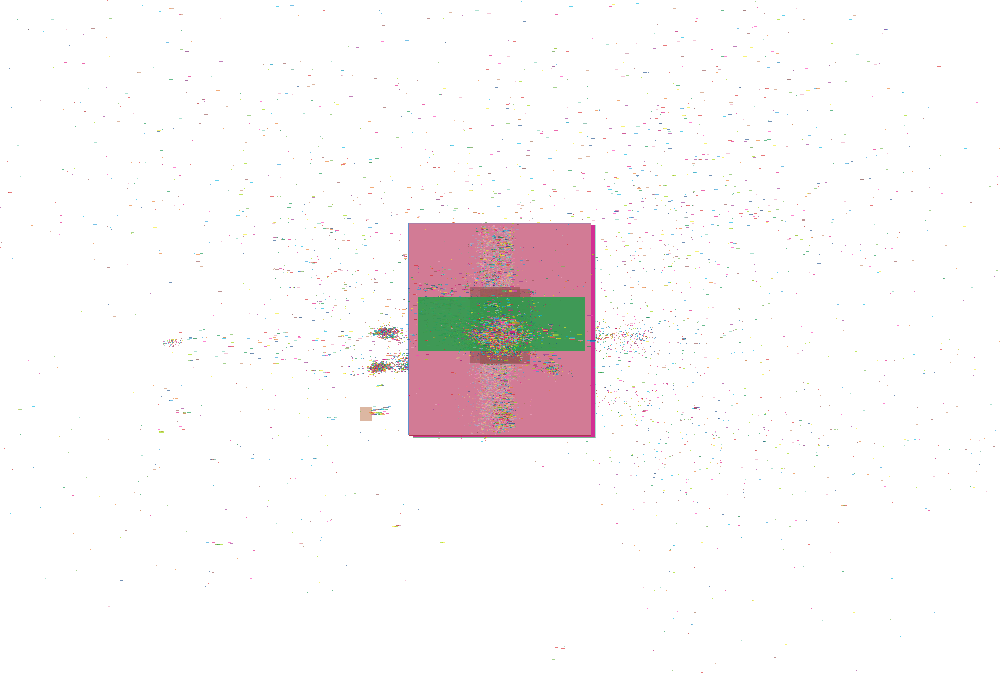
\includegraphics[width=\textwidth, frame]{baseline/convergence_Chip1_LSE_10_gamma.png}
  \caption{\(T_{\NLSE_\gamma}\) with \(\gamma = 10^1\)}
 \end{subfigure}
 \hfill
 \begin{subfigure}{.48\textwidth}
  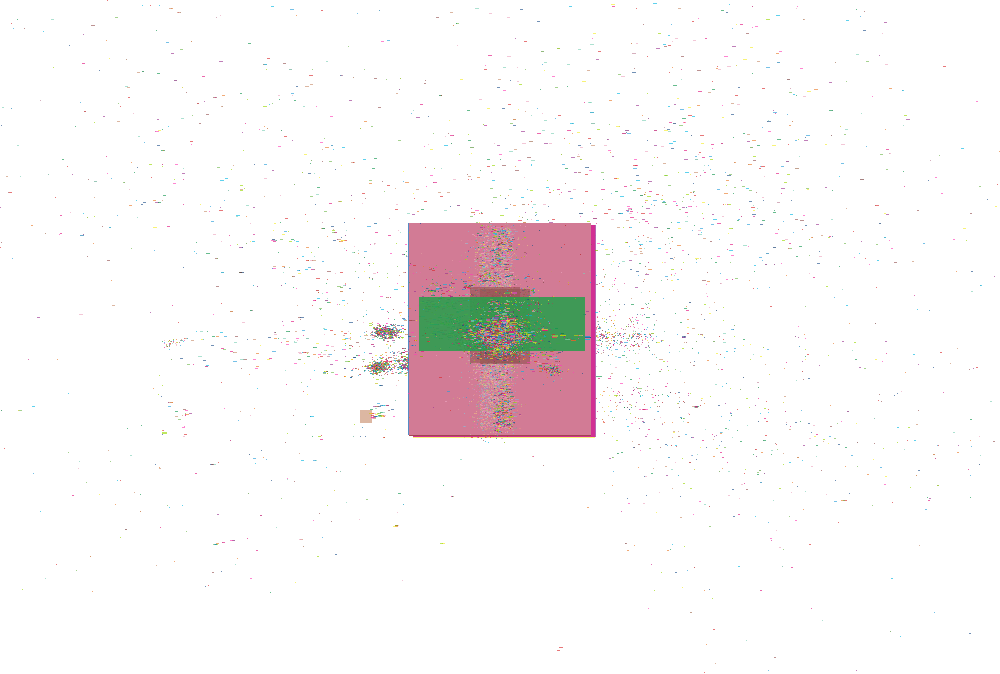
\includegraphics[width=\textwidth, frame]{baseline/convergence_Chip1_WA_10_gamma.png}
  \caption{\(T_{\NWA_\gamma}\) with \(\gamma = 10^1\)}
 \end{subfigure}
 
 \bigskip
 
 \begin{subfigure}{.48\textwidth}
  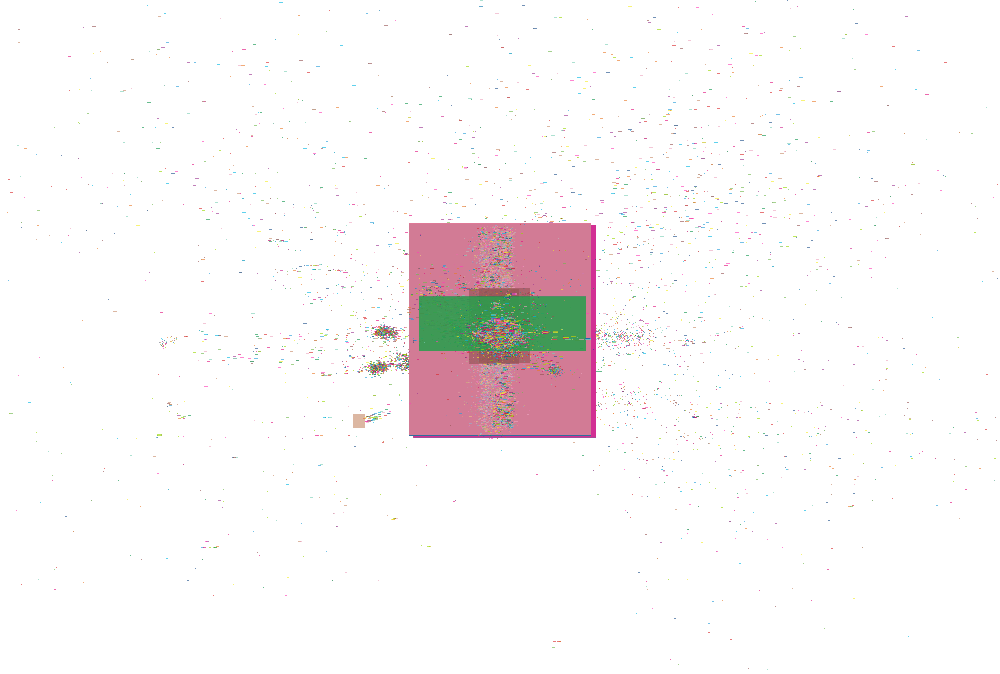
\includegraphics[width=\textwidth, frame]{baseline/convergence_Chip1_LSE_1000_gamma.png}  
  \caption{\(T_{\NLSE_\gamma}\) with \(\gamma = 10^3\)}
 \end{subfigure}
 \hfill
 \begin{subfigure}{.48\textwidth}
  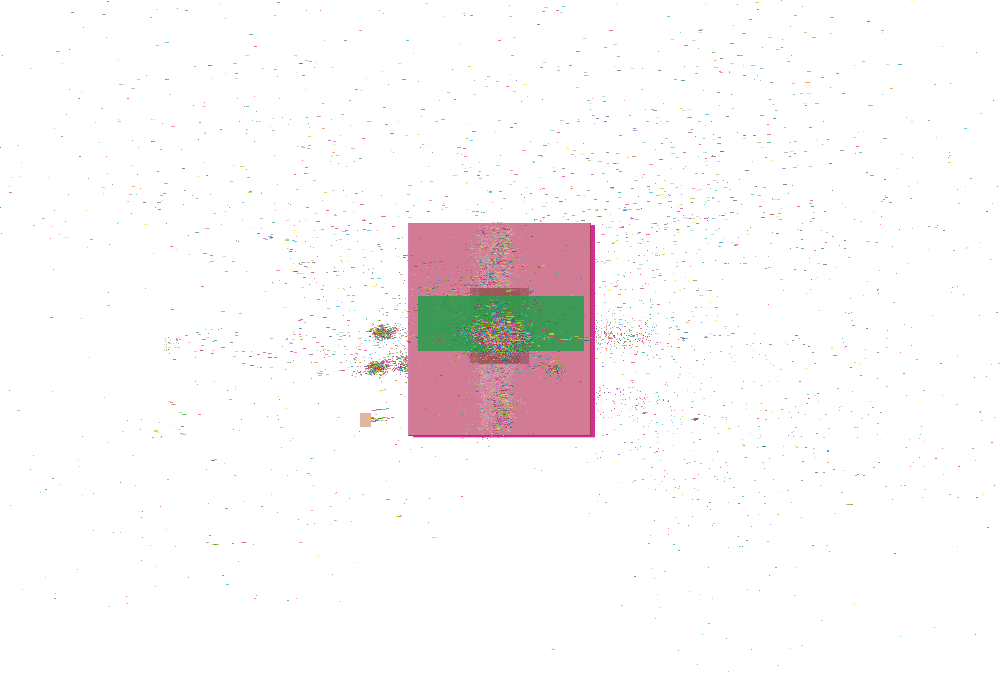
\includegraphics[width=\textwidth, frame]{baseline/convergence_Chip1_WA_1000_gamma.png}  
  \caption{\(T_{\NWA_\gamma}\) with \(\gamma = 10^3\)}
 \end{subfigure}
 
 \bigskip
 
 \begin{subfigure}{.48\textwidth}
  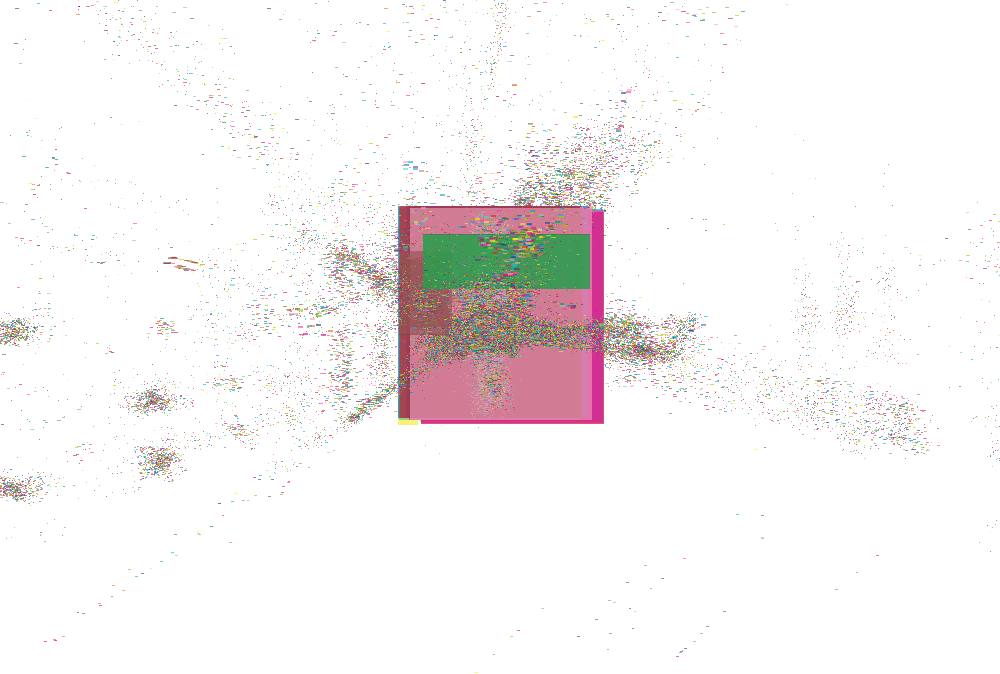
\includegraphics[width=\textwidth, frame]{baseline/convergence_Chip1_LSE_100000_gamma.png}  
  \caption{\(T_{\NLSE_\gamma}\) with \(\gamma = 10^5\)}
 \end{subfigure}
 \hfill
 \begin{subfigure}{.48\textwidth}
  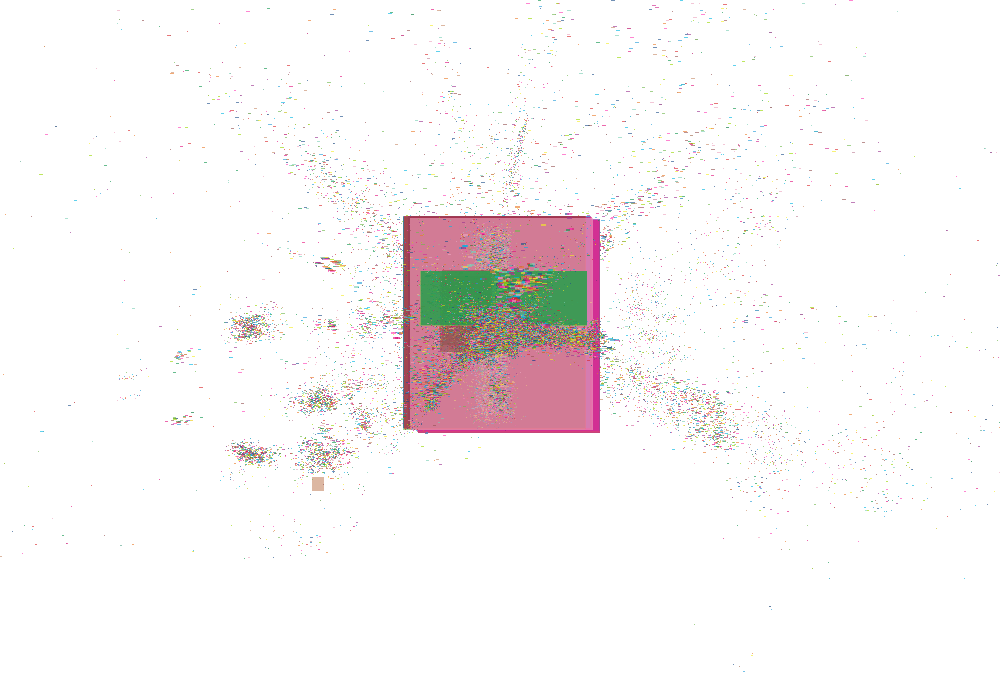
\includegraphics[width=\textwidth, frame]{baseline/convergence_Chip1_WA_100000_gamma.png}  
  \caption{\(T_{\NWA_\gamma}\) with \(\gamma = 10^5\)}
 \end{subfigure}
 
 \caption{Placement plots after 1000 NAG iterations using the specified objective function, cropped to enlarge the center}
 \label{fig:baseline_placement_plots}
\end{figure}

Qualitative insights about the solution qualities of these methods
can be gained by inspecting the final placements
that are produced by the six objective functions in \cref{fig:baseline_placement_plots}.
All placements look useful in giving insights about relative positions of the cells.
There is no visible difference between the upper four placements
because of how close the objective functions are to each other.
Only when \(\gamma\) becomes big enough the cells start to spread more over the chip area.
While the difference between the plots for \(\NLSE_\gamma\) and \(\NWA_\gamma\) for \(\gamma = 10^5\)
is not easily discernable, the right one places more cells close to the center
of the chip.

To get a quantitative comparison between the different netlength estimations,
the following table lists the evaluation of each netlength estimation (in meters)
for the result of optimizing each objective function.
The objective functions based on \(\NLSE_\gamma\) and \(\NWA_\gamma\)
were optimized as described above so the resulting placements might not be close to optimal.
The objective functions using \(\HPWL\) or \(\QCLIQUE\) were optimized
by solving a MinCostFlow problem with the network simplex algorithm 
or a quadratic program with the conjugate gradient method respectively.
How to construct the MinCostFlow problem and the quadratic program is covered in \cite[pp. 5-7]{BrennerVygen-AnalyticalMethodsInVlsiPlacement}
and will not be discussed here.
The last line of \cref{table:baseline_netlength_estimation_by_objective_function} which is labeled with \enquote{CENTER}
does not correspond to an objective function that is minimized 
but just describes the process of placing all movable cells at the center of the chip area.
This shows how small the estimated total wirelengths can get without using any information about the problem instance
and without gaining any insights about the optimal cell positions.

\begin{table}[h]
 \centering
 \begin{tabular}{c c | r r r r r r r r r r}
               &                   & \(\HPWL\) & \(\NLSE\)   & \(\NWA\)    & \(\NLSE\)   & \(\NWA\)    & \(\NLSE\)    & \(\NWA\) \\
               & \(\gamma =\)      &           & \(10^1\)    & \(10^1\)    & \(10^3\)    & \(10^3\)    & \(10^5\)     & \(10^5\) \\
  \hline
  \(\HPWL\)    &                   & 4.020     & 4.032       & 4.019       & 5.663       & 3.951       & 197.509      & 3.643    \\
  \(\NLSE\)    & \(10^1\)          & 7.144     & 7.146       & 7.143       & 8.128       & 6.913       & 179.292      & 3.731    \\
  \(\NWA\)     & \(10^1\)          & 7.568     & 7.571       & 7.567       & 8.511       & 7.347       & 179.309      & 3.767    \\
  \(\NLSE\)    & \(10^3\)          & 7.357     & 7.357       & 7.357       & 7.999       & 6.962       & 179.248      & 3.658    \\
  \(\NWA\)     & \(10^3\)          & 7.761     & 7.761       & 7.761       & 8.524       & 7.392       & 179.327      & 3.794    \\
  \(\NLSE\)    & \(10^5\)          & 10.016    & 10.016      & 10.016      & 10.356      & 9.720       & 178.669      & 3.447    \\
  \(\NWA\)     & \(10^5\)          & 9.164     & 9.164       & 9.163       & 9.522       & 8.853       & 178.917      & 3.295    \\
  \(\QCLIQUE\) &                   & 8.690     & 8.691       & 8.689       & 9.693       & 8.425       & 178.517      & 3.723    \\
  CENTER       &                   & 5.346     & 5.350       & 5.345       & 6.838       & 5.182       & 180.344      & 4.626    \\
 \end{tabular}
 \caption{Evaluation of the weighted sum of each netlength estimation (column) after optimizing different objective functions (row) in meters}
 \label{table:baseline_netlength_estimation_by_objective_function}
\end{table}

First of all, the table shows how close the objective functions are to \(T_{\HPWL}\) when \(\gamma\) is small
and how far off they are when \(\gamma\) is big.
The second ovservation is that
optimizing with \(\gamma = 10^5\) leads to very low values of the optimized objective function (close to the lowest values in their respective columns)
which is not the case for \(\gamma \leq 10^3\) where the objective function is lowest when optimizing \(T_{\HPWL}\)
but at the same time choosing the lowest \(\gamma\)-value leads to the best results when measured with \(T_{\HPWL}\).

\begin{table}[ht]
 \centering
 \begin{tabular}{c c c c c c}
  \multicolumn{2}{c}{Netlength estimation} & \multicolumn{2}{c}{Total [h:mm:ss]} & \multicolumn{2}{c}{Average iteration [\si{\second}]} \\
               &                           & \(\mathbf{x}\)   & \(\mathbf{y}\)   & \(\mathbf{x}\)   & \(\mathbf{y}\)  \\
  \hline
  \(\HPWL\)    &                           & 4:10:18          & 4:48:33          &                  &        \\
  \(\NLSE\)    & \(\gamma = 10^1\)         & 2:20:16          & 2:20:16          & 8.416            & 8.416  \\
  \(\NLSE\)    & \(\gamma = 10^3\)         & 2:18:35          & 2:17:55          & 8.315            & 8.275  \\
  \(\NLSE\)    & \(\gamma = 10^5\)         & 2:18:22          & 2:17:43          & 8.302            & 9.263  \\
  \(\NWA\)     & \(\gamma = 10^1\)         & 2:58:34          & 2:58:31          & 10.714           & 10.711 \\
  \(\NWA\)     & \(\gamma = 10^3\)         & 2:41:38          & 2:41:38          & 9.698            & 9.698  \\
  \(\NWA\)     & \(\gamma = 10^5\)         & 2:46:01          & 2:46:00          & 9.961            & 9.960  \\
  \(\QCLIQUE\) &                           & 0:00:42          & 0:00:42          &                  &        \\
 \end{tabular}
 \caption{Runtime of optimizing different objective functions}
 \label{table:baseline_runtime_by_objective_function}
\end{table}

The last aspect of this baseline we want to look at is its runtime.
Because x- and y-coordinates are optimized independently both runtimes are shown.
Dividing the total runtime by 1000 gives the time that an average iteration needs.
This can help to determine how many iterations are feasible.
\cref{table:baseline_runtime_by_objective_function} shows those figures for all
the objective functions.
It shows that \(\NLSE\) and \(\NWA\) are vastly slower than \(\QCLIQUE\)
but still faster than determining a \(\HPWL\)-optimal placement.
There are two factors to keep in mind:
Firstly, 1000 iterations are plenty.
It is probably possible that much fewer than 1000 iterations suffice for a reasonable placement.
Secondly, the \texttt{backtracking-line-search} step size strategy is the most expensive of all step size strategies
because it requires at least one additional evaluation of the objective function in each iteration,
so the runtime of an average iteration will also decrease once we explore other step size strategies.
The generally higher runtime of \(\NWA\) is probably caused by the more complicated evaluation of the gradient
while the differences between different \(\gamma\)-values remain unclear.


To summarize, this baseline case leads to the following observations
\begin{enumerate}
 \item The higher \(\gamma\) is the better are the convergence properties and placements
 \item The lower \(\gamma\) is the closer the netlength estimations are to \(\HPWL\)
 \item Optimizing \(\NLSE\) is faster but optimizing \(\NWA\) leads to lower \(\HPWL\)
 \item Even after 1000 iterations the resulting \(\HPWL\) is more than 50\% above the optimum
       when starting with random cell positions
\end{enumerate}
